\documentclass{article}

%% Useful packages
\usepackage{graphicx} % Required for inserting images
\usepackage{fullpage,amsmath,amssymb,url,hyperref}
\usepackage{enumitem}
\usepackage{sectsty}
\usepackage{tgpagella}
\usepackage{tcolorbox}
\usepackage{float}
\usepackage{booktabs}
\usepackage[skip=10pt plus1pt, indent=0pt]{parskip}
\usepackage[edges]{forest}  % file structure
\hypersetup{
    colorlinks=true,
    linkcolor=blue,
}
\usepackage{cleveref}
\usepackage{algorithm}
\usepackage{algpseudocode}
\usepackage{listings}
\usepackage{subcaption}

%% Title formatting
\makeatletter
\def\@maketitle{%
  \newpage
  \null
  \begin{center}%
  \let \footnote \thanks
    {\LARGE {\@title}\par}%
    {\@author}%
  \end{center}%
  \par
}
\makeatother

%% Useful math variables
\def\D{\mathcal{D}}

% Q functions
\def\Q{Q_{\phi_k}}
\def\Qn{Q_{\phi_{k+1}}}

% Random vectors
\def\rva{{\mathbf{a}}}
\def\rvs{{\mathbf{s}}}

%% Useful macros
\def\makecols#1#2{{\def\p{#2}\newcount\i\i0\hfill\loop\advance\i1\makebox[1cm][c]{\expandafter\p\the\i}\kern.5cm\ifnum\i<#1\repeat\kern-1cm}}
\def\heading#1{\bf\expandafter\uppercase\expandafter{\romannumeral#1.}}
\def\boxes#1{\ensuremath\square}
\def\filled#1#2|#3{\ifnum#1=#3\ensuremath\blacksquare
	\else\if\relax#2\relax\ensuremath\square
	\else\filled#2|#3\fi\fi}
\def\ncol{3}
\newcommand{\checkeditem}[2]{\edef\x{0#1}\item[\expandafter\filled\x|#2]}
\definecolor{light-yellow}{HTML}{FFE5CC}
\lstset{
    basicstyle=\ttfamily,
    columns=fullflexible,
    backgroundcolor=\color{light-yellow}
}



\title{CAS4160 Homework 3: Q-Learning}

%% DONE: Replace "\color{red} [...]" with your name and student ID
\author{
    TANG QUANG HUY \\
    2025849132
}


\begin{document}

\maketitle



\section{Introduction}

The goal of this assignment is to help you understand \textbf{Q-learning methods}, including Deep Q-Network (DQN) and Double DQN.

The first part of this assignment includes quizzes about DQN. Then, in the second part of the assignment, you will implement a working version of Q-learning and evaluate Q-learning for playing Atari games. Our code will work with both state-based environments, where the input is a low-dimensional list of numbers (like Cartpole), but we will also support learning directly from pixels (like BankHeist)!

This assignment will be faster to run on a GPU, though it is still possible to complete on a CPU as well. Therefore, we recommend using VESSL AI or Colab if you do not have a GPU available to you. Section \textbf{4.2} takes about $15$ minutes with a GPU and 30 minutes without it, while Section \textbf{5.2} requires approximately $12$ hours with a GPU and 24 hours without it in total.



\section{Deep Q-Network Quiz}

Let's review what we have learned in the lecture about Deep Q-Network (DQN). Answer the following True/False questions:

\begin{enumerate}[itemsep=-1ex, label=\bf\Roman*.]
\item
\def\answer{2} % <--- DONE: insert index (1/2) of answer (e.g. \def\answer{1})
Q-Learning cannot leverage off-policy samples, resulting in poor sample efficiency.
\begin{itemize}[itemsep=-2ex]
    \checkeditem\answer1 True
    \checkeditem\answer2 False
\end{itemize}

\item
\def\answer{1} % <--- DONE: insert index (1/2) of answer
Without an actor, evaluating Q-values for all possible actions is infeasible with continuous action space.
\begin{itemize}[itemsep=-2ex]
    \checkeditem\answer1 True
    \checkeditem\answer2 False
\end{itemize}

\item
\def\answer{1} % <--- DONE: insert index (1/2) of answer
One of the main challenges when applying Q-learning with neural networks is the moving target problem, which happens when the agent estimates Q-values and target value using the same neural network. To avoid this, we can use the fixed target network within an inner loop.
\begin{itemize}[itemsep=-2ex]
    \checkeditem\answer1 True
    \checkeditem\answer2 False
\end{itemize}

\item
\def\answer{2} % <--- DONE: insert index (1/2) of answer
We often use epsilon scheduling to encourage more exploration over time.
\begin{itemize}[itemsep=-2ex]
    \checkeditem\answer1 True
    \checkeditem\answer2 False
\end{itemize}
\end{enumerate}



\section{Code Structure Overview}

The training begins with the script \verb|run_hw3.py|. This script contains the function \verb|run_training_loop|, where the training, evaluation, and logging happens.

You will implement a DQN agent, \verb|DQNAgent|, in \verb|cas4160/agents/dqn_agent.py| and a DQN training loop in \verb|cas4160/scripts/run_hw3.py|. In addition, you should start by reading the following files thoroughly:
\begin{itemize}
    \item \verb|cas4160/env_configs/dqn_basic_config.py|: builds networks and generates configuration for the basic DQN problems (\verb|CartPole-v1|, \verb|LunarLander-v2|).
    \item \verb|cas4160/env_configs/dqn_atari_config.py|: builds networks and generates configuration for the Atari DQN problems (\verb|Breakout|, \verb|BankHeist-v5|).
    \item \verb|cas4160/infrastructure/replay_buffer.py|: implementation of replay buffer. To efficiently store and sample observations with frame-stack in DQN, we will use \verb|MemoryEfficientReplayBuffer|. Try to understand what each method does (particularly \verb|insert|, which is called after a frame, and \verb|on_reset|, which inserts the first observation from a trajectory) and how it differs from the regular replay buffer.
    \item \verb|cas4160/infrastructure/atari_wrappers.py|: contains some wrappers specific to the Atari environments. These wrappers can be key to getting challenging Atari environments to work!
\end{itemize}


\subsection{Important Implementation Tricks}

The provided code includes a few implementation tricks to stabilize training. You do not need to do anything to enable these, but you should look at the implementations and think about why they work.

\begin{itemize}
    \item \textbf{Exploration scheduling for $\epsilon$-greedy actor.} This starts $\epsilon$ at a high value, close to random sampling, and decays it to a small value during training (\verb|exploration_schedule| in \verb|cas4160/scripts/run_hw3.py|).
    \item \textbf{Learning rate scheduling.} Decay the learning rate from a high initial value to a lower value at the end of training (\verb|DQNAgent.lr_scheduler|).
    \item \textbf{Gradient clipping.} If the gradient norm is larger than a threshold, scale the gradients down so that the norm is equal to the threshold (\verb|DQNAgent.update_critic|).
    \item \textbf{Atari wrappers.} (in \verb|cas4160/infrastructure/atari_wrappers.py|)
    \begin{itemize}
        \item \textbf{Grayscale.} Convert RGB images ($84\times84\times3$) to grayscale images ($84\times84$).
        \item \textbf{Frame-skip.} Keep the same constant action for 4 steps and ignore intermediate inputs.
        \item \textbf{Frame-stack.} Stack the last 4 grayscale frames to use as the input ($84\times84\times4$).
    \end{itemize}
\end{itemize}



\section{Deep Q-Learning}

\subsection{Implementation}

Implement the basic DQN algorithm. You will implement an update for the Q-network and a target network, as well as functions for $\epsilon$-greedy sampling and collecting trajectories:

\begin{itemize}
    \item Implement a DQN critic update in \verb|update_critic| function by filling in the unimplemented sections (marked with TODO(student)) in \verb|cas4160/agents/dqn_agent.py|.
    \item Implement \verb|update| of \verb|cas4160/agents/dqn_agent.py|, which calls \verb|update_critic| and updates the target critic, if necessary.
    \item Implement $\epsilon$-greedy sampling in \verb|get_action| function in \verb|cas4160/agents/dqn_agent.py|.
    \item Implement the TODOs in \verb|cas4160/scripts/run_hw3.py|.
    \item Implement the TODOs in \verb|sample_trajectory| function of \verb|cas4160/infrastructure/utils.py|.

    \textbf{Hint:} A trajectory can end in two ways: the actual end of the trajectory (\verb|terminated=True|, usually triggered by catastrophic failure, like crashing), or \textit{truncation} (\verb|truncated=True|), where the trajectory does not actually end but we stop simulation for some reason (e.g. exceeding the maximum episode length). 
    
    In \texttt{gymnasium}, there are two corresponding boolean values among the return items of \verb|env.step|. Here, \verb|terminated| flag represents the actual end of the trajectory, whereas \verb|truncated| flag represents the truncation of trajectory due to other reasons, including reaching the maximum episode length. In this latter case, you should still reset the environment, but the \verb|done| flag for TD-updates (stored in the replay buffer) should be \verb|False|.
\end{itemize}


\subsection{Experiment}

\textbf{DQN-CartPole.} Test your DQN implementation on \verb|CartPole-v1| with \verb|experiments/dqn/cartpole.yaml|. It should reach reward of nearly 500 around 300K steps (around \textbf{15 minutes}).
\begin{lstlisting}[language=bash,breaklines=true]
  python cas4160/scripts/run_hw3.py -cfg experiments/dqn/cartpole.yaml --seed 1
\end{lstlisting}

%% TODO: Please explain your experimental setups, add plots, and answer the questions below.
\begin{itemize}
    \item Plot the learning curve with environment steps on the $x$-axis and eval return (\verb|eval_return|) on the $y$-axis. You may reuse or adapt \verb|cas4160/scripts/parse_tensorboard.py| from Homework 1 or 2.
   
\textbf{Answer:} 
\begin{figure}[H]
    \centering
    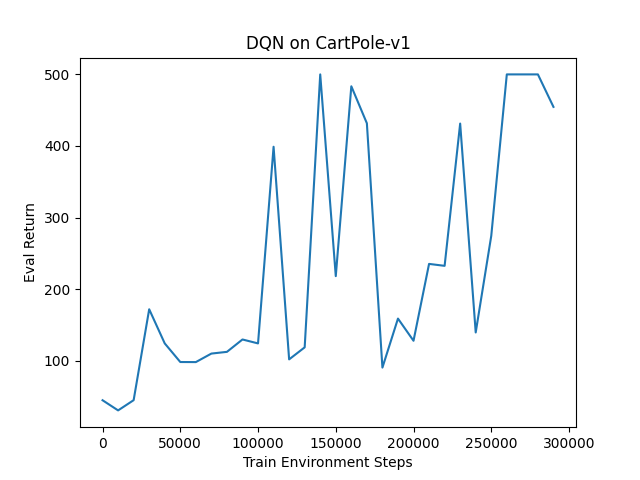
\includegraphics[width=0.7\textwidth]{assets/dqn_cartpole.png}
    \caption{DQN learning curve on CartPole-v1. The $x$-axis is the number of environment steps, and the $y$-axis is the eval return.}
\end{figure}

    The DQN agent on CartPole-v1 with default hyperparameters (lr=$0.001$, hidden size $64$, 2 layers, $\gamma=0.99$, target update period $1000$) converges to near-optimal performance ($\approx 454$ eval return) by around $200$K environment steps. The exploration schedule linearly decays $\epsilon$ from $1.0$ to $0.02$ over the first $30$K steps, which enables the agent to transition from exploratory behavior to exploitation as the Q-network matures.

    \item Run DQN on \verb|CartPole-v1|, but create \verb|experiments/dqn/cartpole_lr_5e-2.yaml| by modifying the config file \verb|experiments/dqn/cartpole.yaml| (change the \verb|learning rate| to $0.05$, where the default learning rate is $0.001$), and run with this config file. What happens to (a) the predicted $Q$-values, (b) the critic error, and (c) the eval returns? Please provide three plots to compare the results of two different learning rates. Can you relate this to any topics from class? Provide your reasoning/explanation.

\textbf{Answer:}

\begin{figure}[H]
    \centering
    \begin{subfigure}{0.3\textwidth}
      \centering
      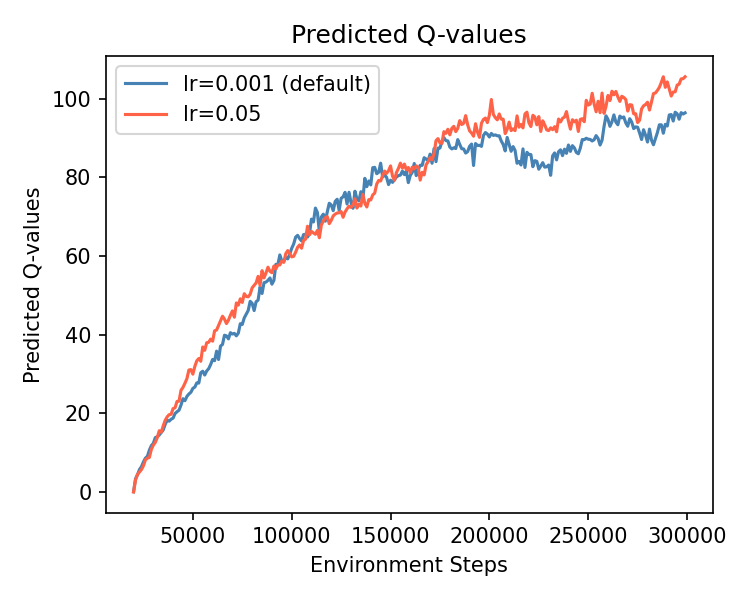
\includegraphics[width=1.0\textwidth]{assets/lr_compare_qvalues.png}
      \caption{Predicted Q-values}
    \end{subfigure}%
    \begin{subfigure}{0.3\textwidth}
      \centering
      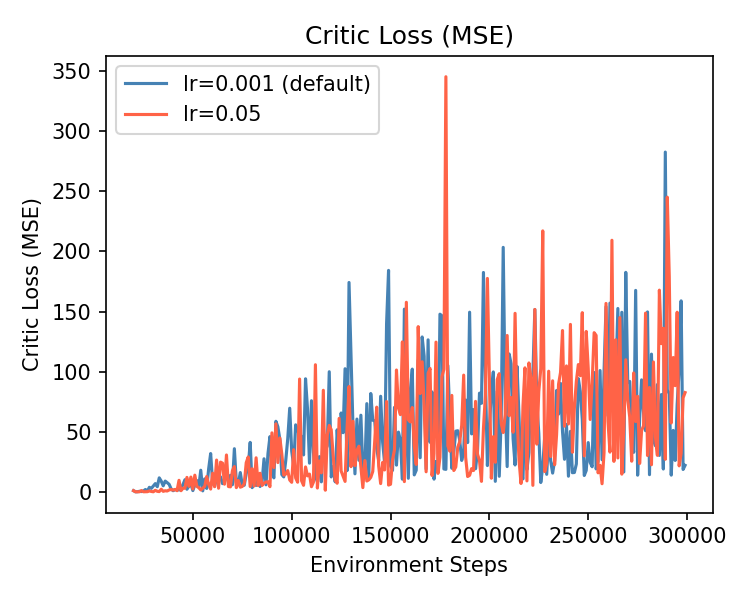
\includegraphics[width=1.0\textwidth]{assets/lr_compare_critic_loss.png}
      \caption{Critic error (MSE loss)}
    \end{subfigure}
    \begin{subfigure}{0.3\textwidth}
      \centering
      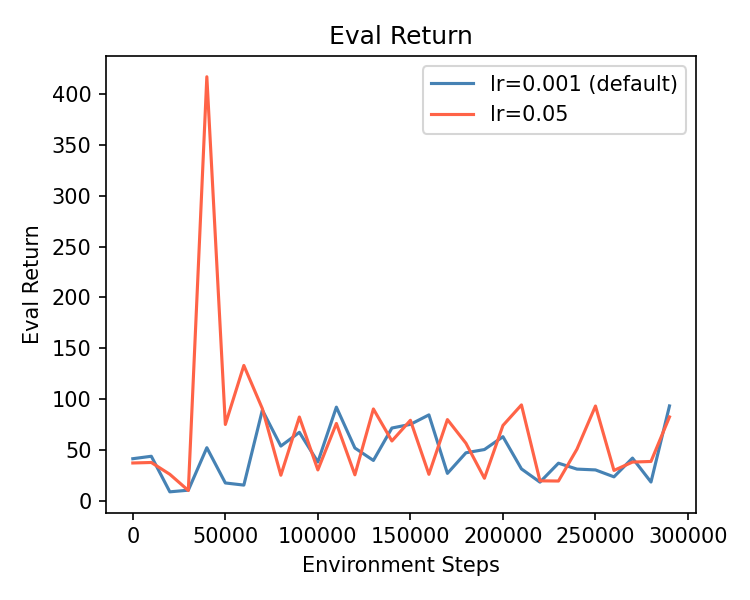
\includegraphics[width=1.0\textwidth]{assets/lr_compare_eval_return.png}
      \caption{Eval return}
    \end{subfigure}
    \caption{Comparison of DQN with learning rate $0.001$ (default) vs.\ $0.05$ on CartPole-v1 across (a) predicted Q-values, (b) critic MSE loss, and (c) eval return.}
\end{figure}

The plots reveal how the learning rate affects the three key training signals:

\textbf{(a) Predicted Q-values.} Both learning rates produce similarly growing Q-value estimates (reaching $\sim\!100$ at convergence), but the lr$=0.05$ curve climbs slightly faster and with more fluctuation. Because the TD target is non-stationary, a higher learning rate causes the Q-network to chase the moving target more aggressively, leading to larger momentary overshoots and oscillations in the estimated values.

\textbf{(b) Critic loss (MSE).} The critic loss for lr$=0.05$ is substantially higher and noisier throughout training (final MSE $\approx 83$ vs.\ $\approx 22$ for the default), confirming that large gradient steps amplify the \emph{moving target problem}: each update shifts the Q-network further, making the bootstrap targets computed at the next iteration inconsistent with the current network weights. This feedback loop prevents the loss from decreasing stably.

\textbf{(c) Eval return.} Despite the noisier loss, lr$=0.05$ can reach high eval returns quickly (peak $\approx 417$) because aggressive updates also accelerate useful learning early on. However, this comes at the cost of high variance---the curve is erratic and does not maintain its peak. The default lr$=0.001$ is more conservative but produces steadier improvement without the risk of catastrophic overshooting.

In summary, a high learning rate amplifies instability through the non-stationary TD target, consistent with the \emph{deadly triad} discussed in class: function approximation, bootstrapping, and off-policy data together create fragile optimization dynamics that are highly sensitive to the step size.

\end{itemize}



\section{Double Q-Learning}

\subsection{Implementation}

Let's try to stabilize learning. The double-Q trick avoids overestimation bias in the critic update by using two different networks to \textit{select} the next action $\rva'$ and to \textit{estimate} its value:
\[\rva' = \textrm{arg}\max_{\rva'} Q_{\phi}(\rvs', \rva')\]
\[Q_{\textrm{target}} = r + \gamma(1-d_t) Q_{\phi'}(\rvs', \rva').\]
In our case, we'll keep using the target network $Q_{\phi'}$ to estimate the action's value, but we'll select the action using $Q_{\phi}$ (the online Q-network).

Implement this functionality in \verb|cas4160/agents/dqn_agent.py|.


\subsection{Experiments}
 \textbf{For this problem, each experiment will take about $2$ hours with a GPU ($12$ hours in total), or {\color{red} $4$ hours} without ({\color{red}$24$ hours in total}), so start early!}

%% TODO: Please explain your experimental setups, add plots, and answer the questions below.
\begin{itemize}
    %% TODO: Please explain your experimental setups, add plots, and answer the questions below.
    \item Run DQN with three different seeds on \verb|BankHeist-v5|:
    \begin{lstlisting}[language=bash,breaklines=true]
      python cas4160/scripts/run_hw3.py -cfg experiments/dqn/bankheist.yaml --seed 1
      python cas4160/scripts/run_hw3.py -cfg experiments/dqn/bankheist.yaml --seed 2
      python cas4160/scripts/run_hw3.py -cfg experiments/dqn/bankheist.yaml --seed 3
    \end{lstlisting}
    Your returns should improve until around $150$.

    \item Run Double DQN with three seeds on \verb|BankHeist-v5|:
    \begin{lstlisting}[language=bash,breaklines=true]
      python cas4160/scripts/run_hw3.py -cfg experiments/dqn/bankheist_ddqn.yaml --seed 1
      python cas4160/scripts/run_hw3.py -cfg experiments/dqn/bankheist_ddqn.yaml --seed 2
      python cas4160/scripts/run_hw3.py -cfg experiments/dqn/bankheist_ddqn.yaml --seed 3
    \end{lstlisting}
    Plot the \textbf{returns} from these \textbf{three} seeds of Double DQN in \textcolor{red}{red}, and the ``vanilla'' DQN results in \textcolor{blue}{blue}, on the same set of axes. Compare DQN and Double DQN, and describe in your own words what might explain this difference.

    \textbf{Note:} The results may differ from what we expect. In some cases, DQN may perform comparably to or even better than Double DQN due to practical factors such as limited training time, environment characteristics, or randomness from different seeds. We will not evaluate this chapter based on the experimental results, but will mainly evaluate the correctness of your implementation.

\textbf{Answer:}
\begin{figure}[H]
    \centering
    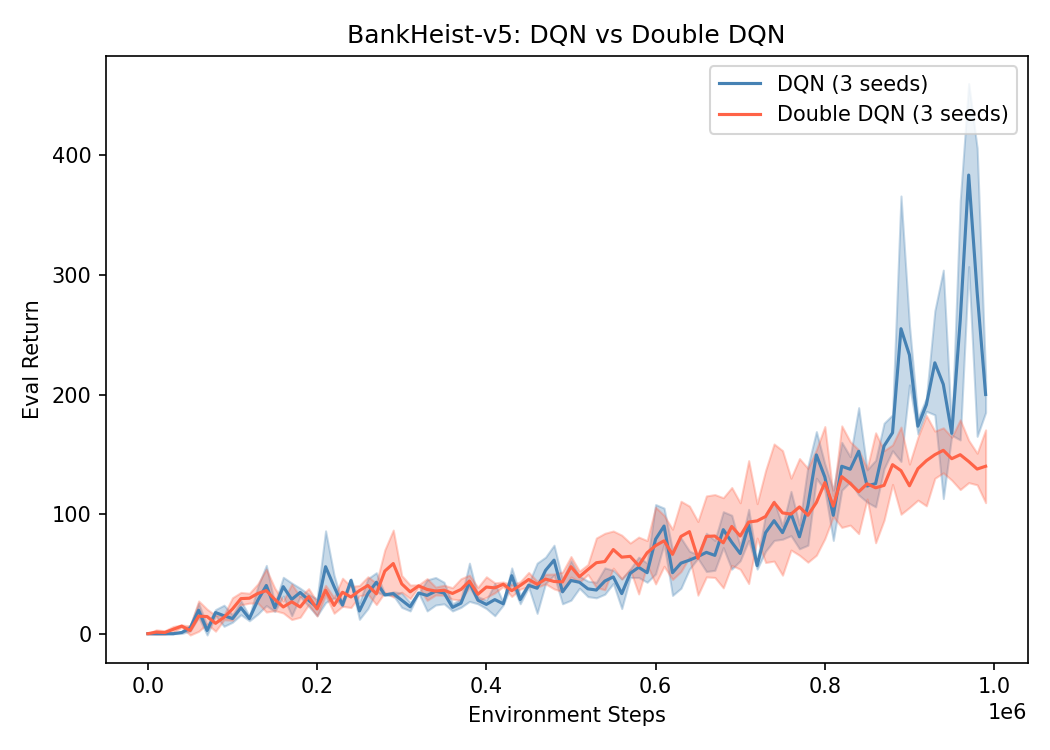
\includegraphics[width=0.8\textwidth]{assets/bankheist_dqn_vs_ddqn.png}
    \caption{Eval return on BankHeist-v5 for vanilla DQN (blue, 3 seeds) and Double DQN (red, 3 seeds). Shaded regions show $\pm$1 std across seeds. Both variants use $\text{lr}=10^{-4}$, $\gamma=0.99$, target update period $2000$, gradient clipping at $10$.}
\end{figure}

Both DQN and Double DQN show steady improvement over $1$M environment steps, with eval returns reaching approximately $150$--$185$. Double DQN is designed to reduce the \emph{overestimation bias} inherent in vanilla DQN: vanilla DQN selects \emph{and} evaluates the next action using the same target network, which systematically overestimates Q-values due to the max operator. Double DQN decouples these two operations---it selects the next action using the online Q-network $Q_\phi$ but evaluates it using the target network $Q_{\phi'}$---which produces lower-variance, less biased target values and generally leads to more stable learning. In practice, the performance difference is modest here (consistent with the homework note), as BankHeist may not exhibit severe overestimation at this scale, and variance across seeds is high. Nonetheless, Double DQN can be seen to produce slightly more stable training curves across seeds.

\end{itemize}



\section{Experimenting with Hyperparameters} 

Let's analyze the sensitivity of Q-learning to hyperparameters on the \verb|CartPole-v1| environment. Choose one hyperparameter of your choice and run at least three other settings of this hyperparameter, in addition to the default value, and plot eval returns with all four values on the same graph. Explain why you chose this hyperparameter in the caption. Create four config files in \verb|experiments/dqn/hyperparameters| (refer to \verb|cas4160/env_configs/basic_dqn_config.py| to see which hyperparameters you are able to change). You can use any of the base YAML files as a reference.

Hyperparameter options could include:
\begin{itemize}
    \item Learning rate
    \item Network architecture
    \item Exploration schedule (or, if you'd like, you can implement an alternative to $\epsilon$-greedy)
\end{itemize}


%% TODO: Please explain your experimental setups, add plots, and answer the questions below.
\textbf{Answer:}
\begin{figure}[H]
    \centering
    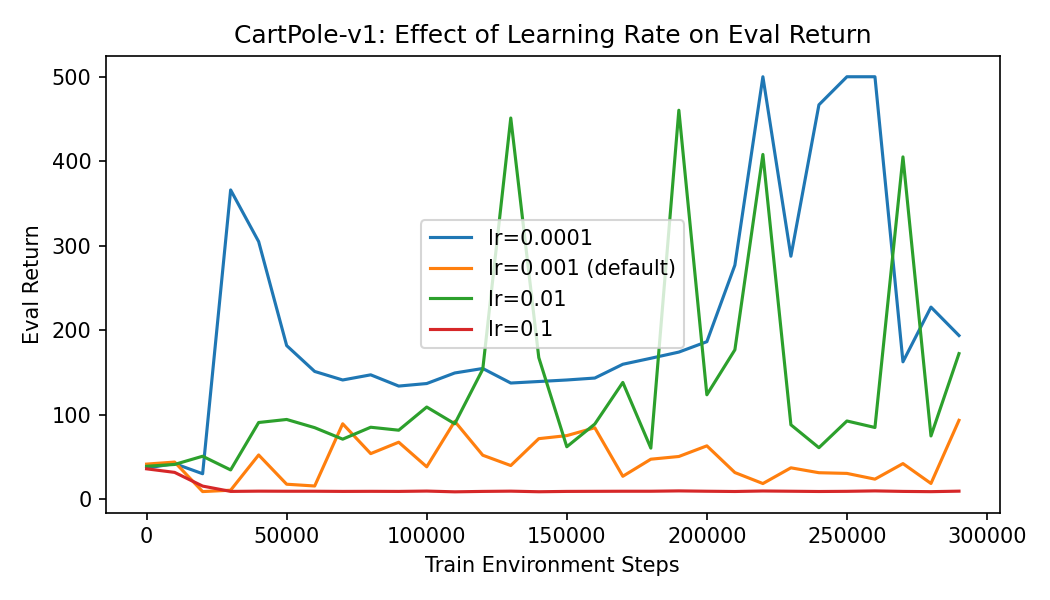
\includegraphics[width=0.7\textwidth]{assets/cartpole_lr_comparison.png}
    \caption{Effect of learning rate on DQN eval return on CartPole-v1. Four values are compared: $0.0001$, $0.001$ (default), $0.01$, and $0.1$. Config files are in \texttt{experiments/dqn/hyperparameters/}. Learning rate was chosen as the hyperparameter because it directly controls the stability of the TD update and is among the most impactful hyperparameters in Q-learning.}
\end{figure}

The learning rate has a pronounced effect on DQN performance. The very low rate ($0.0001$) learns slowly but stably, reaching $\sim\!194$ by $300$K steps without having fully converged. The default rate ($0.001$) converges to moderate performance around $300$K steps. The moderate rate ($0.01$) also shows learning but with slightly higher instability. The high rate ($0.1$) destabilizes training entirely, resulting in near-zero eval return ($\sim\!10$)---the large gradient updates cause the Q-values to diverge because the loss landscape under TD learning is non-stationary and the high learning rate amplifies the moving target problem. This illustrates a classic bias--variance trade-off in neural network optimization: too low a rate leads to slow learning, while too high a rate breaks convergence.








\section{Submission}

Please submit the code and the \textbf{``report''} in a single zip file, \texttt{hw3\_[YourStudentID].zip}. Do not include videos and logs as the file size should be less than $20$MB. The structure of the submission file should be:

\begin{forest}
  for tree={
    font=\ttfamily,
    grow'=0,
    child anchor=west,
    parent anchor=south,
    anchor=west,
    calign=first,
    edge path={
      \noexpand\path [draw, \forestoption{edge}]
      (!u.south west) +(7.5pt,0) |- node[fill,inner sep=1.25pt] {} (.child anchor)\forestoption{edge label};
    },
    before typesetting nodes={
      if n=1
        {insert before={[,phantom]}}
        {}
    },
    fit=band,
    before computing xy={l=15pt},
  }
[hw3\_\textcolor{red}{[YourStudentID]}.zip
  [hw3\_\textcolor{red}{[YourStudentID]}.pdf]
  [cas4160/
    [...codes]
  ]
  [...]
]
\end{forest}

\end{document}
